\chapter{The first Chapter}
\label{ch:Chapter_1}
    \graphicspath{{Chapter_1_Folder/figures/PNG/}{Chapter_1_Folder/figures/PDF/}{Chapter_1_Folder/figures/}}

An example citation \cite{pdg} 

\section{A section}

{\small
\begin{center}
\begin{savenotes}
\begin{tabular}{cccccc}
Field & Description & \pbox{20cm}{\relax\ifvmode\centering\fi
Gauge \\\vspace{-2pt}boson} & \pbox{20cm}{\relax\ifvmode\centering\fi
$\su{3}$ \\\vspace{-2pt}representation} & \pbox{20cm}{\relax\ifvmode\centering\fi
$\su{2}$\\\vspace{-2pt}representation} & \pbox{20cm}{\relax\ifvmode\centering\fi
$\uone$\\\vspace{-2pt}Hypercharge} \\
\hline
$B$	& Weak hypercharge	& $\mathrm{B}^0$ & $\mathbf{1}$ & $\mathbf{1}$ & 0 \\
$W$	& Weak isospin			& $\mathrm{W}^\pm, \mathrm{W}^0$ & $\mathbf{1}$ & $\mathbf{3}$ & 0 \\
$G$ & Colour				& Gluons & $\mathbf{8}$ & $\mathbf{1}$ & 0 \\
\hline
$Q_{\mathrm{L}}$ &	Left-handed quark		&& $\mathbf{3}$ & $\mathbf{2}$ & $\frac{1}{6}$ \\
$u_{\mathrm{R}}$ &	Left-handed up quark	&& $\mathbf{3}$ & $\mathbf{1}$ & $\frac{2}{3}$ \\
$d_{\mathrm{R}}$ &	Left-handed down quark	&& $\mathbf{3}$ & $\mathbf{1}$ & $-\frac{1}{3}$ \\
$L_{\mathrm{L}}$ &	Left-handed lepton		&& $\mathbf{1}$ & $\mathbf{2}$ & $-\frac{1}{2}$ \\
$E_{\mathrm{R}}$ &	Right-handed electron	&& $\mathbf{1}$ & $\mathbf{1}$ & $-1$ \\
\hline
$H$ &	Elementary Higgs\footnote{It is the introduction of the elementary Higgs (also known as the \emph{Standard Model Higgs}) here which takes us from the Standard Model to the Minimal Standard Model}	&& $\mathbf{1}$	& $\mathbf{2}$	& $\frac{1}{2}$
\end{tabular}
\end{savenotes}
\end{center}
}

An example footnote \footnote{Hi, I am a footnote.}
\subsection{A subsection.}









\begin{figure}[htb]
	\center
	\begin{subfigure}[b]{0.4\textwidth}
		\center
		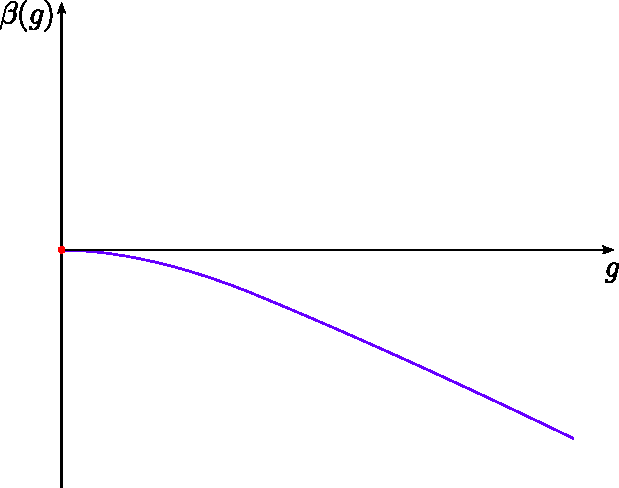
\includegraphics[width=\textwidth]{beta-confining.pdf}
		\subcaption{Confining}
	\end{subfigure}
	\qquad
	\begin{subfigure}[b]{0.4\textwidth}
		\center
		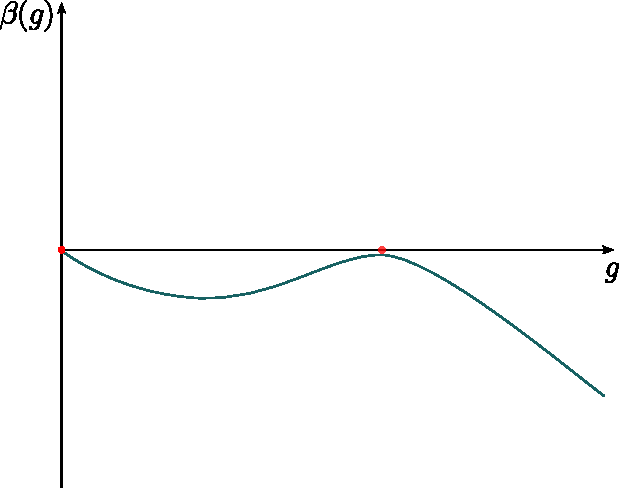
\includegraphics[width=\textwidth]{beta-nearconformal.pdf}
		\subcaption{Near-conformal}
		\label{fig:beta-nearconformal}
	\end{subfigure}


	\begin{subfigure}[b]{0.4\textwidth}
		\center
		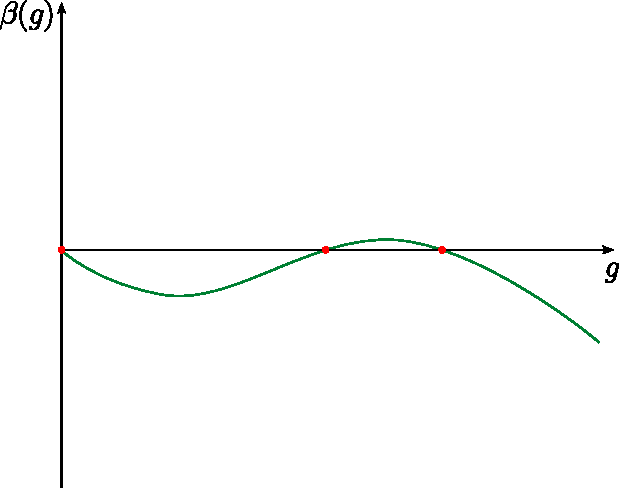
\includegraphics[width=\textwidth]{beta-conformal.pdf}
		\subcaption{Conformal}
	\end{subfigure}
	\qquad
	\begin{subfigure}[b]{0.4\textwidth}
		\center
		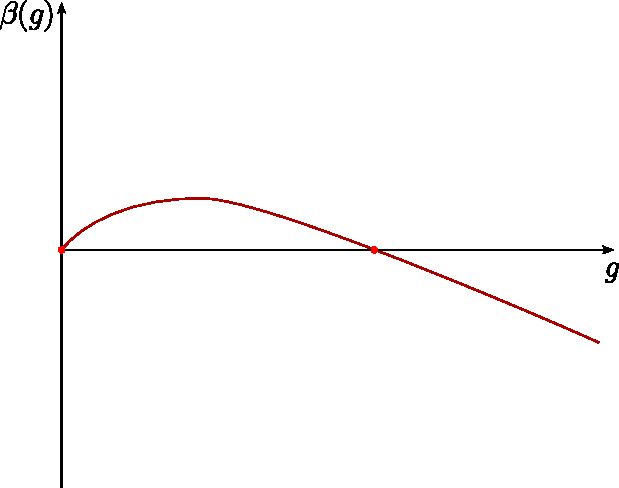
\includegraphics[width=\textwidth]{beta-coulomb.pdf}
		\subcaption{Asymptotic freedom lost}
	\end{subfigure}	
	\caption{Sketches of the $\beta$ function in each of the regions discussed in the text.}
\end{figure}

\begin{figure}[htb]
	\center
	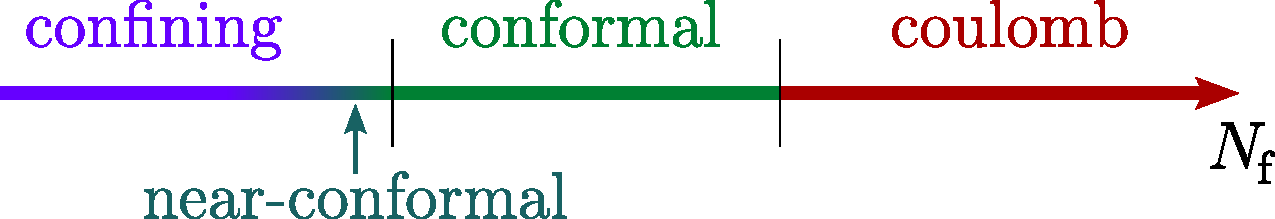
\includegraphics[width=0.5\columnwidth]{phasediagram.pdf}
	\caption{A cartoon showing the cases of theory one encounters as $\Nf$ is varied.}
	\label{fig:phasediag}
\end{figure}

